\documentclass{beamer}
\usepackage{ctex}
\usepackage{hyperref}
\usepackage[T1]{fontenc}

% other packages
\usepackage{latexsym}
\usepackage{amsmath}
\usepackage{xcolor}
\usepackage{multicol}
\usepackage{booktabs}
\usepackage{calligra}
\usepackage{graphicx}
\usepackage{pstricks}
\usepackage{listings}
\usepackage{stackengine}
\usepackage{caption}
\usepackage{verbatim}
\usepackage{makecell}
\usepackage{ulem}

\author{陈文轩}
\title{基于Nios II 实现多类型LCD屏幕彩条显示}
\subtitle{电子信息虚拟仿真实验期末汇报}
\institute{杭州电子科技大学卓越学院}
\date{2025年5月12日}
\usepackage{HDU}

% defs
\def\cmd#1{\texttt{\color{red}\footnotesize $\backslash$#1}}
\def\env#1{\texttt{\color{blue}\footnotesize #1}}
\definecolor{deepblue}{rgb}{0,0,0.5}
\definecolor{deepred}{rgb}{0.5,0,0}
\definecolor{deepgreen}{rgb}{0,0.5,0}
\definecolor{halfgray}{gray}{0.7}

\lstset{
	basicstyle=\ttfamily\small,
	keywordstyle=\bfseries\color{deepblue},
	emphstyle=\ttfamily\color{deepred},    % Custom highlighting style
	stringstyle=\color{deepgreen},
	numbers=left,
	numberstyle=\small\color{halfgray},
	rulesepcolor=\color{red!20!green!20!blue!20},
	frame=shadowbox,
}


\begin{document}
	
	\kaishu
	\begin{frame}
		\titlepage
		\begin{figure}[htpb]
			\begin{center}
				
\includegraphics[width=0.35\linewidth]{pic/HDUlogo.pdf}
			\end{center}
		\end{figure}
	\end{frame}
	
	%生成目录
	\begin{frame}
		\tableofcontents[sectionstyle=show,subsectionstyle=show/shaded/hide,subsubsectionstyle=show/shaded/hide]
	\end{frame}
	
	
	
\section{实验基本原理}
	
	
	
\begin{frame}{Qsys/NiosII简介}
    \begin{itemize}[<+-| alert@+>]
    \item 利用Qsys系统集成工具,通过IP核简单搭建SOPC系统,并自动创建IP核(如SDRAM的控制)之间的互联逻辑(例化、互相通信等)。

    \item NiosII是Altera为FPGA设计的一种RSIC架构的嵌入式软核处理器。NiosII作为处理器核心,是Qsys中可以使用的众多IP之一。

    \item Qsys提供图形化界面设计系统,NiosII则提供软件开发环境运行程序(嵌入式C语言开发)
     \end{itemize}
\end{frame}

\begin{frame}{实验完成大致流程1}
    \begin{itemize}[<+-| alert@+>]
        \item 根据正点原子NiosII教程,先利用Qsys工具部署IP核,并进行连接。
     \end{itemize}
     \pause
    \centering
    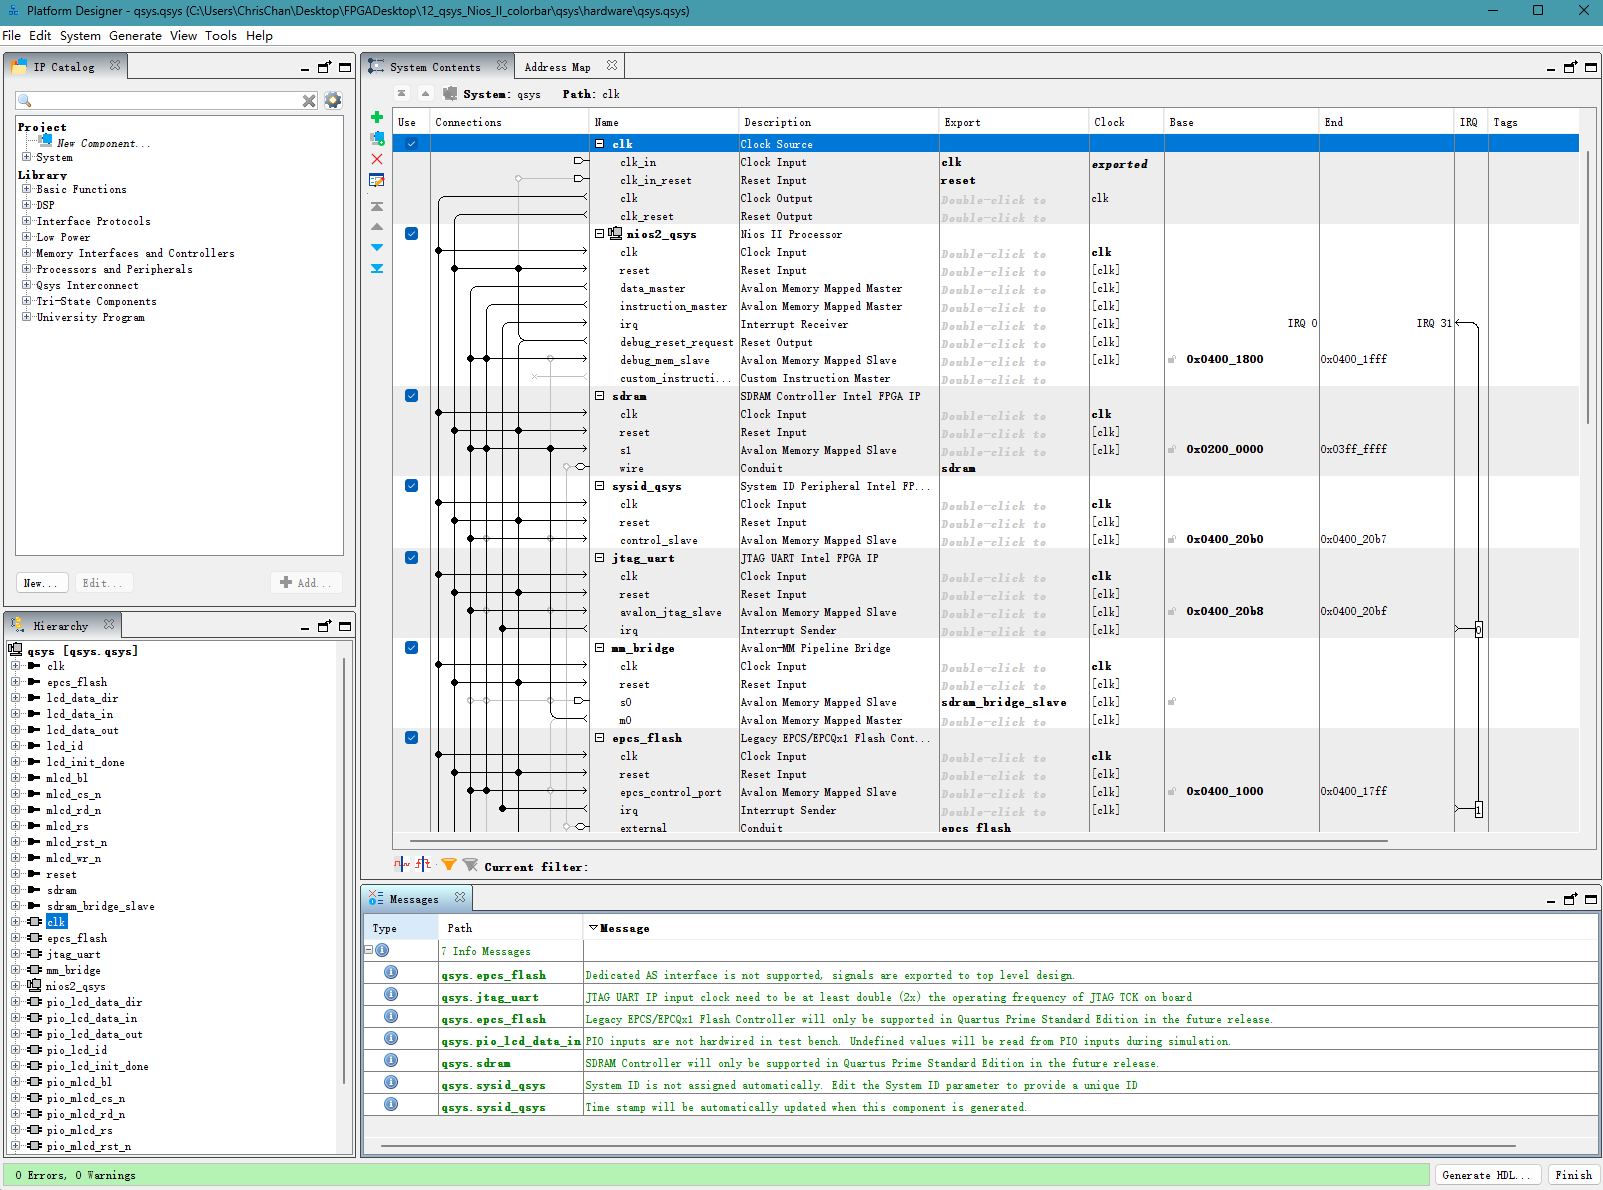
\includegraphics[width=1\textwidth]{pic/004.png}
    \captionof{figure}{Qsys IP核端口连接部署}
    \label{fig:system_block_diagram}

\end{frame}

\begin{frame}{实验完成大致流程2}
    \begin{itemize}[<+-| alert@+>]
        \item 根据正点原子NiosII嵌入式设计教程,设计嵌入式C程序
     \end{itemize}
     \pause
    \centering
    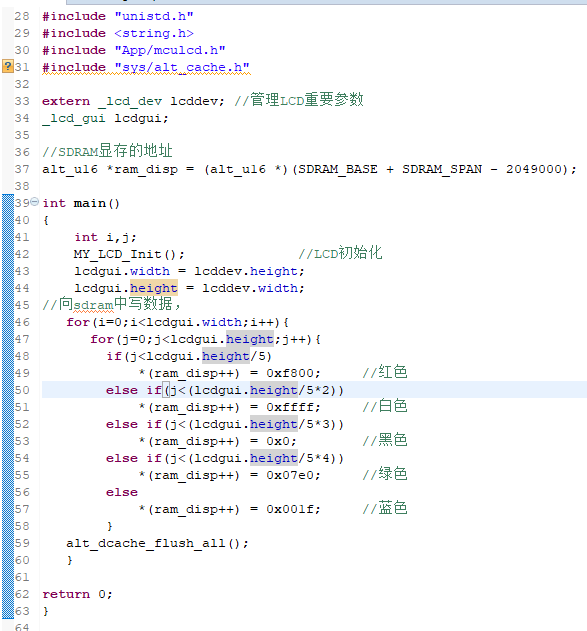
\includegraphics[width=1\textwidth]{pic/003.png}
    \captionof{figure}{实验C代码}
    \label{fig:system_block_diagram}

\end{frame}

\begin{frame}{Qsys实验原理简介}
    \begin{columns}
        % 左侧列放置图片
        \begin{column}{0.5\textwidth}
            \centering
            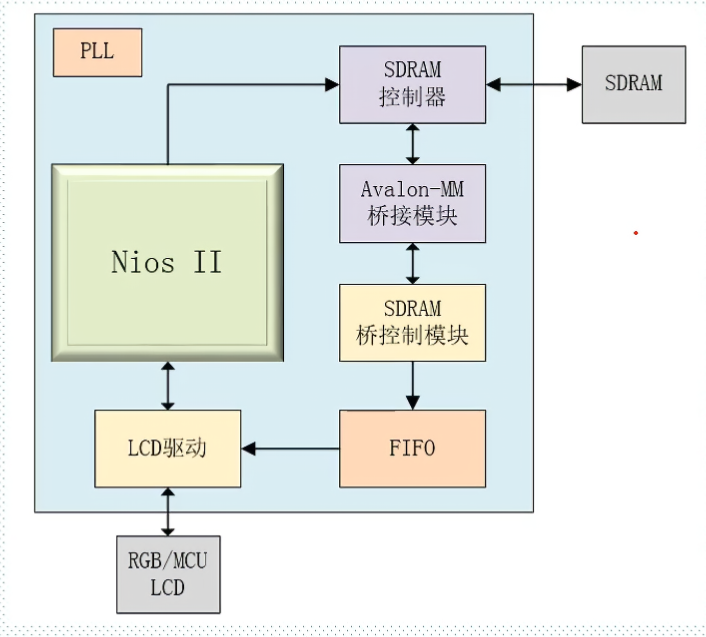
\includegraphics[width=1\textwidth]{pic/001.png}
            \captionof{figure}{实验框图}
            \label{fig:system_block_diagram}
        \end{column}
        
        % 右侧列可以放置文字说明
        \begin{column}{0.5\textwidth}{Qsys主要IP核介绍}
			\begin{itemize}[<+-| alert@+>]
				\item 由于LCD模块是部署在NiosII之外的模块,但也需要读取SDRAM的彩条控制信息
				\item 利用SDRAM控制器IP核的一个Avalon的端口引出
				\item 通过Avalon-MM模块的突发传输功能提高数据吞吐量
				\item 最终实现LCD模块可以高效访问外部SDRAM,即SDRAM控制模块由NiosII和SDRAM桥控制模块两个主机进行控制
			\end{itemize}
        \end{column}
    \end{columns}
\end{frame}



\begin{frame}{LCD驱动实验原理简介}
    \begin{columns}
        % 左侧列放置图片
        \begin{column}{0.5\textwidth}
            \centering
            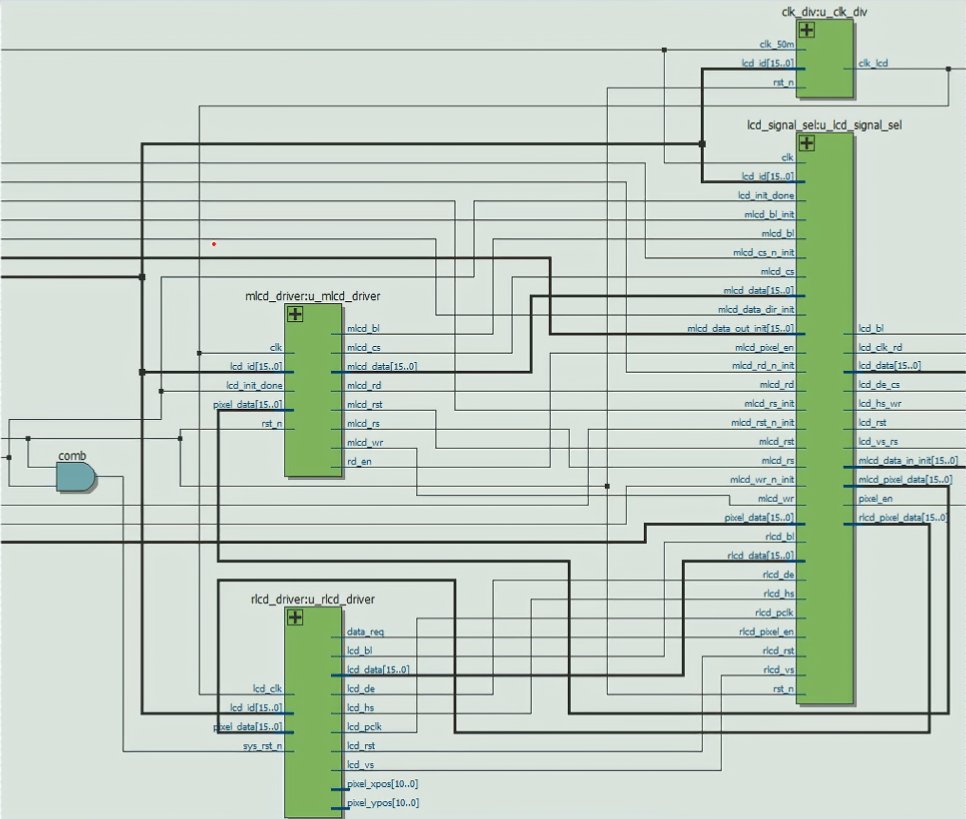
\includegraphics[width=1\textwidth]{pic/002.png}
            \captionof{figure}{实验框图}
            \label{fig:system_block_diagram}
        \end{column}
        
        % 右侧列可以放置文字说明
        \begin{column}{0.5\textwidth}{LCD驱动介绍}
			\begin{itemize}[<+-| alert@+>]
				\item 根据LCDID[15:0]信号,判断出当前的LCD屏幕类型(像素点多少、所需时钟频率等),进行针对化驱动
				\item LCD模块采用的是逐行扫描的形式,具体来说,它通过行计数器(hcnt)和场计数器(vcnt)模拟行同步和场同步信号,从左到右、从上到下依次写入像素数据到LCD的GRAM中,确保图像按顺序刷新显示。
			\end{itemize}
        \end{column}
    \end{columns}
\end{frame}


\begin{frame}{实验程序示例}
    \begin{columns}
        % 左侧列放置C语言代码
        \begin{column}{0.5\textwidth}
            \centering
            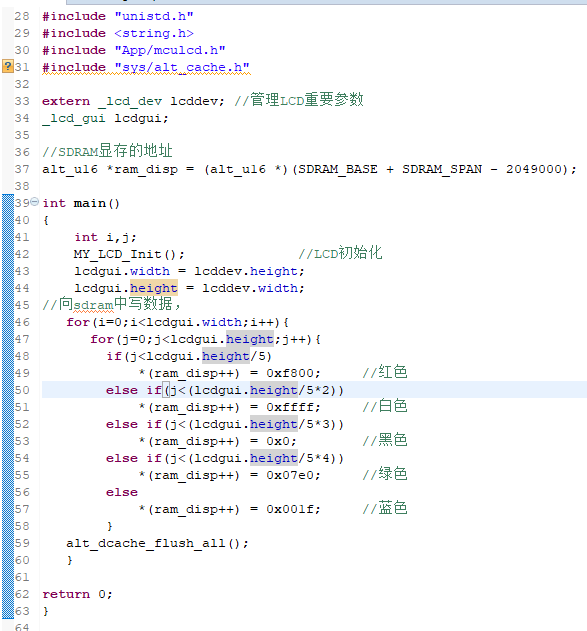
\includegraphics[width=1\textwidth]{pic/003.png}
            \captionof{figure}{实验C代码}
            \label{fig:system_block_diagram}
        \end{column}
        
        % 右侧列放置文字说明
        \begin{column}{0.5\textwidth}
            \begin{itemize}
                \item 该程序初始化 LCD 并设置显存地址。
                \item 使用嵌套循环向 SDRAM 写入彩条数据。
                \item 彩条颜色依次为红、白、黑、绿、蓝。
                \item 使用 `alt\_dcache\_flush\_all` 刷新数据缓存。
            \end{itemize}
        \end{column}
    \end{columns}
\end{frame}




\begin{frame}
	\begin{center}
		{\Huge\calligra Thanks!}
	\end{center}
\end{frame}
	
	
\end{document}
